\def\year{2017}\relax
%File: formatting-instruction.tex
\documentclass[letterpaper]{article} %DO NOT CHANGE THIS
\usepackage{aaai17}  %Required
\usepackage{times}  %Required
\usepackage{helvet}  %Required
\usepackage{courier}  %Required
\usepackage{url}  %Required
\usepackage{graphicx}  %Required
\frenchspacing  %Required
\setlength{\pdfpagewidth}{8.5in}  %Required
\setlength{\pdfpageheight}{11in}  %Required
\usepackage{algorithm}
\usepackage{algorithmic}
\usepackage{amssymb}
\usepackage{graphicx}
\usepackage[caption=false]{subfig}
\graphicspath{ {images/} }
%PDF Info Is Required:
  \pdfinfo{
/Title (Edge Grasp Classification in Deep Learning)
/Author (Dian Wang)}
\setcounter{secnumdepth}{0}  
 \begin{document}
% The file aaai.sty is the style file for AAAI Press 
% proceedings, working notes, and technical reports.
%

\title{Edge Grasp Classification in Deep Learning}
\author{Wang, Dian\\
Northeastern University, Boston, MA\\
{wang.dian@husky.neu.edu}
}
\maketitle
\begin{abstract}
This paper considers the problem of the influence of table edge or shelf edge to robot grasp pose detection in point clouds. Edge grasps, meaning grasps that is pointing to the edge of table or shelf, will not only lower the performance of grasping, but also harm the gripper if collision occurs. Non-edge grasps that is pointing to an actual object is desired in grasping task. An algorithm is produced to take point cloud and grasp configurations as input, and to classify each grasp as either an edge grasp or a non-edge grasp. This paper used two image representation of potential grasps, and two convolutional neural networks is built as classifier, corresponding to the two representations. Experiments were performed to evaluate the performance of this algorithm and compare those two classifiers. The analysis shows that the better classifier reaches a classification accuracy of 88.7\%, and 89.6\% of edge grasps could be removed.
\end{abstract}

\section{Introduction}
\noindent Grasping is one of the most intuitive and the most widely applied technology in robotics. Grasping could be divided into two sub-problems: perception and planning. The robot always needs to observe the environment and determine the target object, then planning technology is applied to operate the robot to reach the grasp configuration. Grasp detection is the base of a grasping task.

Recently, researchers have proposed grasp detection methods that estimate potential grasps independently of object identity. Those methods take RGBD image or point cloud from depth sensor as input and generate output of various grasp configurations. Some of those methods combine the technology in machine learning. Classification methods are used to deal with the RGBD image or point cloud to generate grasp candidates. 

Some of those methods are promising and reliable. \cite{RN6} achieved a 93\% end-to-end grasp success rate for novel objects presented in dense clutter with their grasp pose detection (GPD) method using convolutional neural networks on point cloud data. 

However, one problem of such method is that their algorithm is produced and analyzed in some relatively flat environment such as table top. In practical grasping applications which aim to grasp object on table or shelf, some grasp pointing to the edge of table or shelf may be regarded as good grasp. This will not only influence the performance in grasping task, but also harm the gripper by collision. 

\begin{figure}[t]
    \centering
    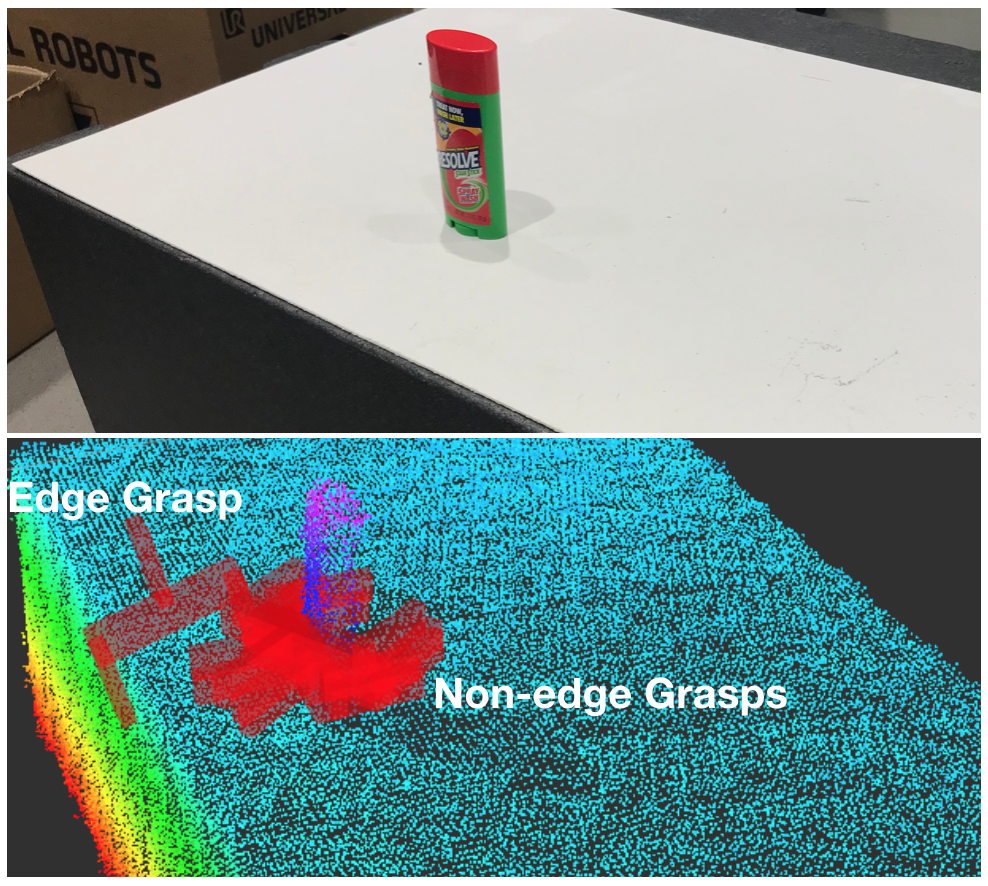
\includegraphics[width=8cm]{images/edgegraspexample.png}
    \caption{A grasping task and grasp candidates. Below is the point cloud of the above environment. The red markers are grasp candidates. One grasp candidate on the left is pointing to the table edge}
    \label{fig:my_label}
\end{figure}

In this paper, a series of methods are proposed to make GPD avoid that problem. First, 2 grasp representation methods are used to transform raw data from point cloud as well as grasp configuration into image that can be used for neural network input. One of the 2 representations is made up of three 2D images, and another is made up of one 3D image. Second, 2 convolutional neural network classifiers are built respectively for those 2 representations. One of them is a 2D CNN classifier for the 2D image, and another is 3D CNN classifier for the 3D image. They take the representation image as input and output the probability for that grasp being edge grasp or non-edge grasp. Data is collected to train these 2 classifiers. Third, experiments are made to evaluate the performance of the 2 classifiers.

\section{Background}

Point cloud is a set of data points in space, each data point in a point cloud contains the information of the position of that point in some reference frame. Point clouds are generally produced by instruments like depth sensor. Point cloud is widely used in computer science, especially in robotics, because it can provide position information of object in space, which RGB data does not have. 

Convolutional neural network (CNN) is a class of deep, feed-forward artificial neural networks that has successfully been applied to analyzing visual imagery. CNNs use a variation of multilayer perceptrons designed to require minimal pre-processing compared to other image classification algorithms. This means that the network learns the filters that in traditional algorithms were hand-engineered. Although CNNs is traditionally used to process images, recently CNNs are widely used in other domains such as Deep Reinforcement Learning and so on.

Grasping involves observing the environment as well as generating potential grasps from observed information. Some grasp detection methods like the ROS grasp pipeline \cite{RN5} build a CAD model of the target object, then calculate a trajectory that grasp the localized object. However, these approaches assume that an accurate CAD model could be built for every grasping object. In contrast, GPD \cite{RN6} detect potential grasps by analyzing the local geometry and/or graspable surface.

\begin{algorithm}[H]
\caption{Grasp Pose Detection}
\textbf{Input:} a view point cloud,  $\mathbb{C}$; a region of interest, $R$; a hand, $\Theta$; a positive integer, $\mathbb{N}$ \\
\textbf{Output:} a set of 6-DOF grasp candidates, $H\subset R$ \\
\begin{algorithmic}[1]
\STATE $\mathbb{C}'={\rm PreprocessCloud}(\mathbb{C})$
\STATE $R={\rm GetROI}(\mathbb{C}')$
\STATE $S={\rm Sample}(\mathbb{C}',R,\Theta, \mathbb{N})$
\STATE $I={\rm Encode}(S,\mathbb{C}', R, \Theta)$
\STATE $H={\rm Score}(I)$
\STATE $g={\rm SelectGrasp}(S, H)$
\end{algorithmic}  
\end{algorithm}  

Their algorithm, as is shown in Algorithm 1, works as follow. Step 1 preprocess the original point cloud. Step 2 characterize the region of interest (ROI), which is the region of the target location. Step 3 samples a series of grasp candidates from ROI. Step 4 encodes each grasp candidate as a multi-channel image. Step 5 assign each candidate a score. Those scores indicate how likely that candidate is a grasp. Step 6 select a number of grasps based on the score from step 5.


\section{Related Work}
\subsection{Choosing Grasp Heuristically}
By manually confine grasp configuration based on the known knowledge of the environment, edge grasps could be avoided to some extent. For example, a "top grasp" \cite{RN8}, which means the gripper approaches the object from the top down, along with the direction of the gravity vector, is always a non-edge grasp since the edge is always perpendicular to the gravity vector. However, this requires enough space above the grasp position. If there is a board on top of the target object, normally "top grasp" is impossible to reach. When there are only "side grasps" (the gripper approaches the object along with some directions that are perpendicular to the gravity vector), the problem still exists.

\subsection{Multi-view Representation of Point Cloud}
One approach to apply convolutional neural networks to point cloud is using multiple view representation of some point cloud. Multi-view CNN \cite{RN7} takes 12 2D images from 12 different views from a 3D shape model as input, outputs object class predictions.
Based on multi-view CNN, GPD used 15 channels image representation for each grasp \cite{RN6}. For each of the x, y, and z axis, they have an averaged height map of the occupied points, an averaged height map of the unobserved region, and 3 averaged surface normal images.

\subsection{Occupancy Grid Representation of Point Cloud}
3D convolutional neural networks are also used when applying convolutional neural networks to point cloud data. VoxNet \cite{RN4} provided a basic 3D CNN architecture that can be applied to create fast and accurate object class detectors for point cloud data. Their method takes point cloud as input, generates occupancy grid based on that point cloud, and uses a 2-layer 3D CNN for classification.

\section{Project Description}
\subsection{Overview of Edge Grasp Classification Algorithm}
Given a point cloud, $\mathbb{C}$, and a transformation matrix, from base frame to hand frame, representing a grasp, ${^h}T_b$, the edge grasp classification problem is to compute the probability $P$, indicating that the input grasp being an edge grasp.

\begin{algorithm}[H]
\caption{Edge Grasp Classification}
\textbf{Input:} a point cloud, $\mathbb{C}$; a grasp transformation matrix, ${^h}T_b$ \\
\textbf{Output:} a probability of that grasp being edge grasp, $P\in [0, 1]$ \\
\begin{algorithmic}[1]
\STATE $I={\rm GraspRepresentation}(\mathbb{C}, {^h}T_b)$
\STATE $P={\rm CNN}(I)$
\end{algorithmic}
\end{algorithm}

My algorithm follows the steps shown in Algorithm 2.  Step 1 encodes the grasp candidate into representation image(s) from the original point cloud and the transformation matrix (from base frame to hand frame) of that grasp. Step 2 generate the probability of that grasp being an edge grasp using convolutional neural network.

\subsection{Grasp Representation}
Each grasp candidate is represented in image(s) of fixed size so that it could be used for the input of convolutional neural network. The image should contain the information of the geometry of the observed grasping surface. Let $\mathbb{C}$ be the observed point cloud in base frame, and ${}^hT_b$ be the transformation matrix of a grasp from base frame to hand frame, then the point cloud in hand frame ${}^h\mathbb{C}$ is:
\begin{equation}
    {}^h\mathbb{C}={}^hT_b\mathbb{C}
\end{equation}
and the points that will be computed into image is:
\begin{equation}
    X=\{\forall {\rm point}\in {}^h\mathbb{C}|{\rm point}\in {\rm ROI}\}
\end{equation}
where ROI is a cubic region of interest.

\subsubsection{Multiple View Representation.}
Inspired by the representation in GPD \cite{RN6} and the idea of multi-view CNN \cite{RN7}, this paper firstly uses a 3-channel multi-view image. Specifically, $X$ is projected onto 3 planes parallel to the 3 axes of the hand frame. For example, the projection of the (x, y) plane is calculated as follows:

For point $X[i]$, its (x, y) coordinates $C(x, y)[i]$ in the projection image is computed as:
\begin{equation}
    C(x, y)[i]=\frac{p-1}{l} (X(x, y)[i] + \frac {l} 2)
\end{equation}
where $X(x, y)[i]$ is the x, y value of point $X[i]$, $p$ is the number of the pixels in the square projection image, and $l$ is the length of the cubic ROI. $C(x, y)[i]\in [0, p)$ and $C(x, y)[i]\in \mathbb{Z}$

The value $V(x, y)[i]$ of point $X[i]$ in the projection image is computed as:
\begin{equation}
    V(x, y)[i]=\frac{X(z)[i]+\frac{l}{2}}{l}
\end{equation}
where $X(z)[i]$ is the z value of point $X[i]$. $V(x, y)[i]\in [0, 1]$. 

After the coordinates and values of each point is computed, the image $I(x, y)$ is computed as:

\begin{algorithm}[H]
\caption{Projection Image for (x, y) Plane}
\textbf{Input:} coordinates $C=C(x, y)$; values $V=V(x, y)$\\
\textbf{Output:} projection image in (x, y) plane, $I=I(x,y)$ \\
\begin{algorithmic}[1]
\FOR {$i = 0 \to p-1$}
\FOR {$j = 0 \to p-1$} 
\STATE $I[i, j] = 0$
\ENDFOR
\ENDFOR
\FOR {$i = 0 \to n$}
\STATE $I[C[i].x, C[i].y]=\max(I[C[i].x, C[i].y], V[i])$
\ENDFOR
\STATE $I={\rm GrayDilation}(I)$
\end{algorithmic}
\end{algorithm}

The value of a particular pixel in the image is the max value of all points that is assigned into the coordinate of that pixel. Gray dilation \cite{BK1} is applied to avoid the influence of void pixels.

After applying above methods to 3 planes parallel to the 3 axis of the hand reference frame, a $3\times p \times p$ image is generated for a grasp candidate.

\subsubsection{3D Occupancy Grid Representation.} This paper also use a 3 dimensional occupancy grid image, where $X$ is transformed into a binary 3D image. The 3D image is calculated as follows:
For point $X[i]$, its coordinates $C'[i]$ in the occupancy image is computed as:
\begin{equation}
    C'[i]=\frac{p-1}{l} (X[i]+\frac{l}{2})
\end{equation}
where $C'[i]\in [0, p)$ and $C'[i]\in \mathbb{Z}$.

The image $I'$ is computed as:
\begin{algorithm}[H]
\caption{Occupancy Image}
\textbf{Input:} coordinates $C'$\\
\textbf{Output:} occupancy image, $I'$\\
\begin{algorithmic}[1]
\FOR {$i = 0 \to p-1$}
\FOR {$j = 0 \to p-1$}
\FOR {$k = 0 \to p-1$}
\STATE $I[i, j, k] = 0$
\ENDFOR
\ENDFOR
\ENDFOR
\FOR {$i = 0 \to n$}
\STATE $I[C[i].x, C[i].y, C[i].z]=1$
\ENDFOR
\STATE $I={\rm BinaryDilation}(I)$
\end{algorithmic}
\end{algorithm}

The value of a particular pixel in the image is 1 if at least 1 point is assigned into the coordinate of that pixel, or the value will be 0. Similarly, binary dilation \cite{BK1} is applied to avoid the influence of void pixels.

After applying above methods, a $p\times p\times p$ image is generated for a grasp candidate.

\subsection{Convolutional Neural Networks}
Convolutional neural networks are applied to computing the probability. This paper use PyTorch \cite{Pytorch} to implement CNNs.

\subsubsection{2.5D CNN for Multiple View Image.} This paper used the basic structure of LeNet \cite{RN3}. The detailed structure is:
\begin{figure}[H]
    \centering
    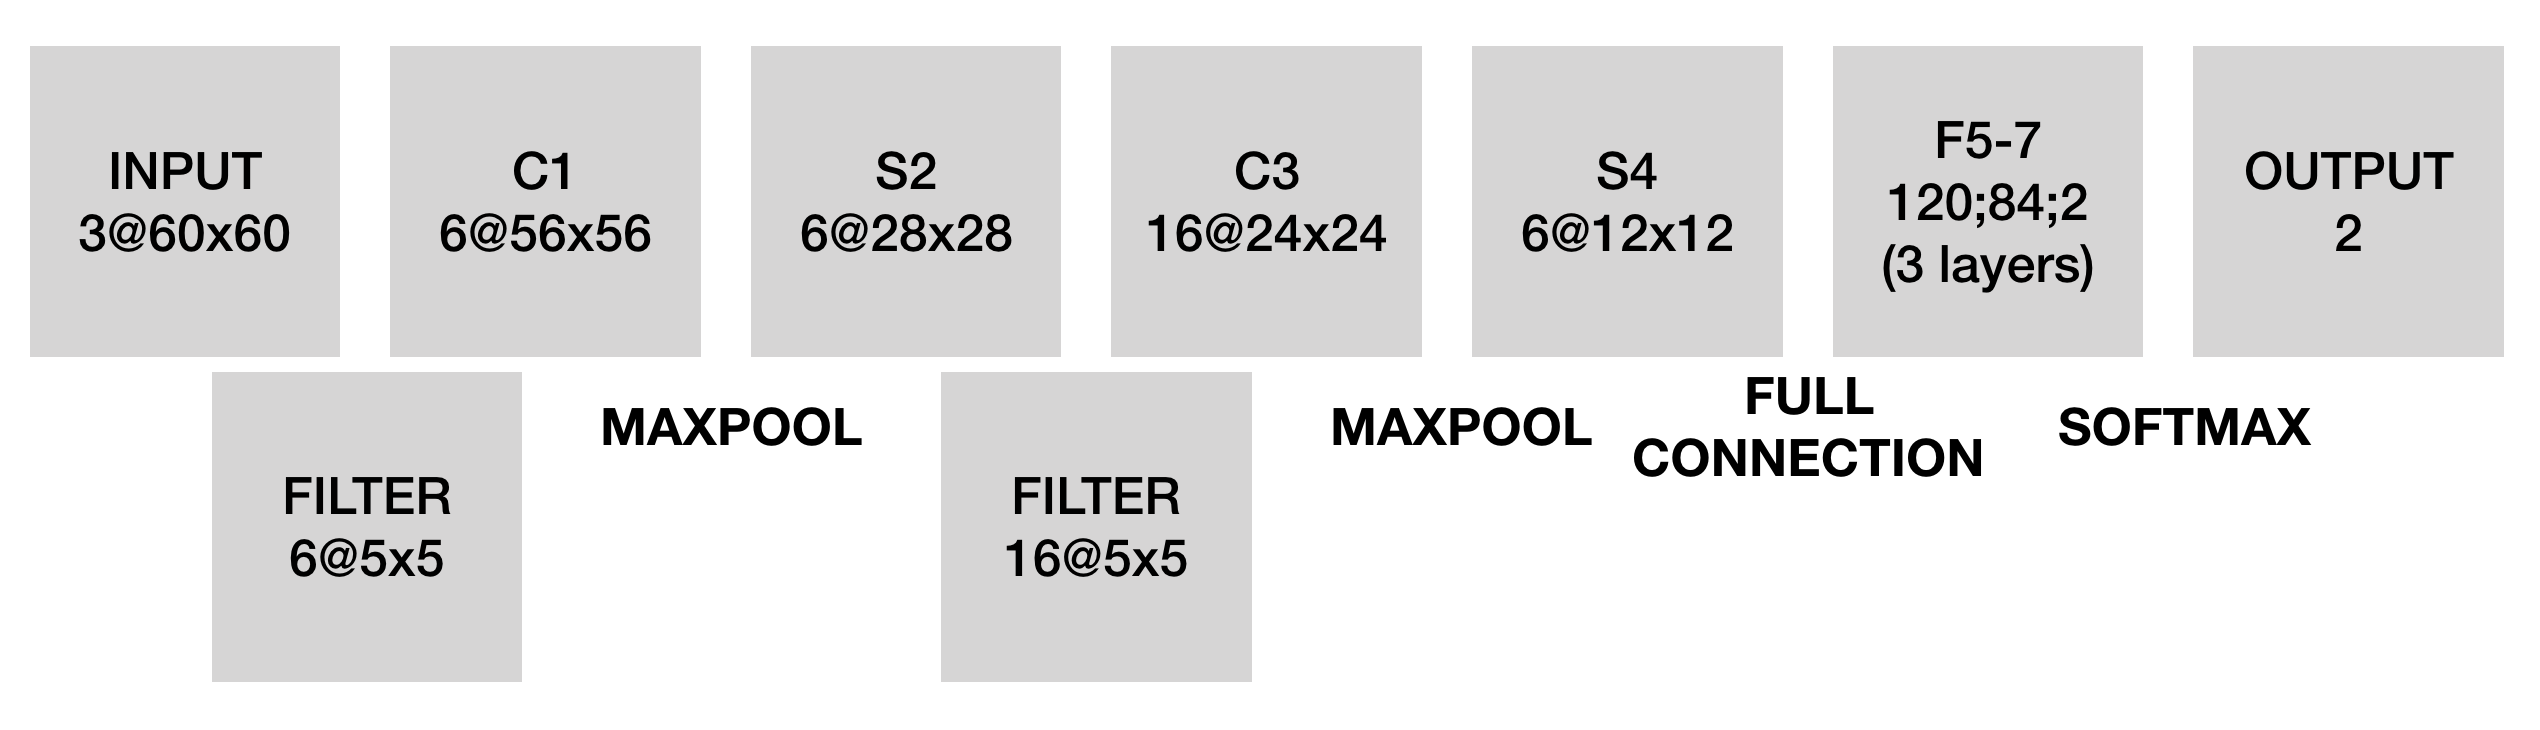
\includegraphics[width=8cm]{images/CNN.png}
    \caption{Structure of CNN}
    \label{fig:my_label}
\end{figure}
The input is $3\times60\times60$ projection image from above multiple view representation. A $6\times5\times5$ filter is applied first, which produce a $6\times56\times56$ hidden layer. The second filter with size $16\times5\times5$ is applied after max pooling, then max pooling again. After that, 3 full connection layer is used, and Softmax function generates the output. The output of this CNN is 2 probabilities, representing the input grasp image being edge grasp and non-edge grasp.

\subsubsection{3D CNN for Occupancy Image.} This paper further applied a 3 dimensional convoluntional neural network to the occupancy grid image. The structure is inspired by VoxNet \cite{RN4}. 
\begin{figure}[H]
    \centering
    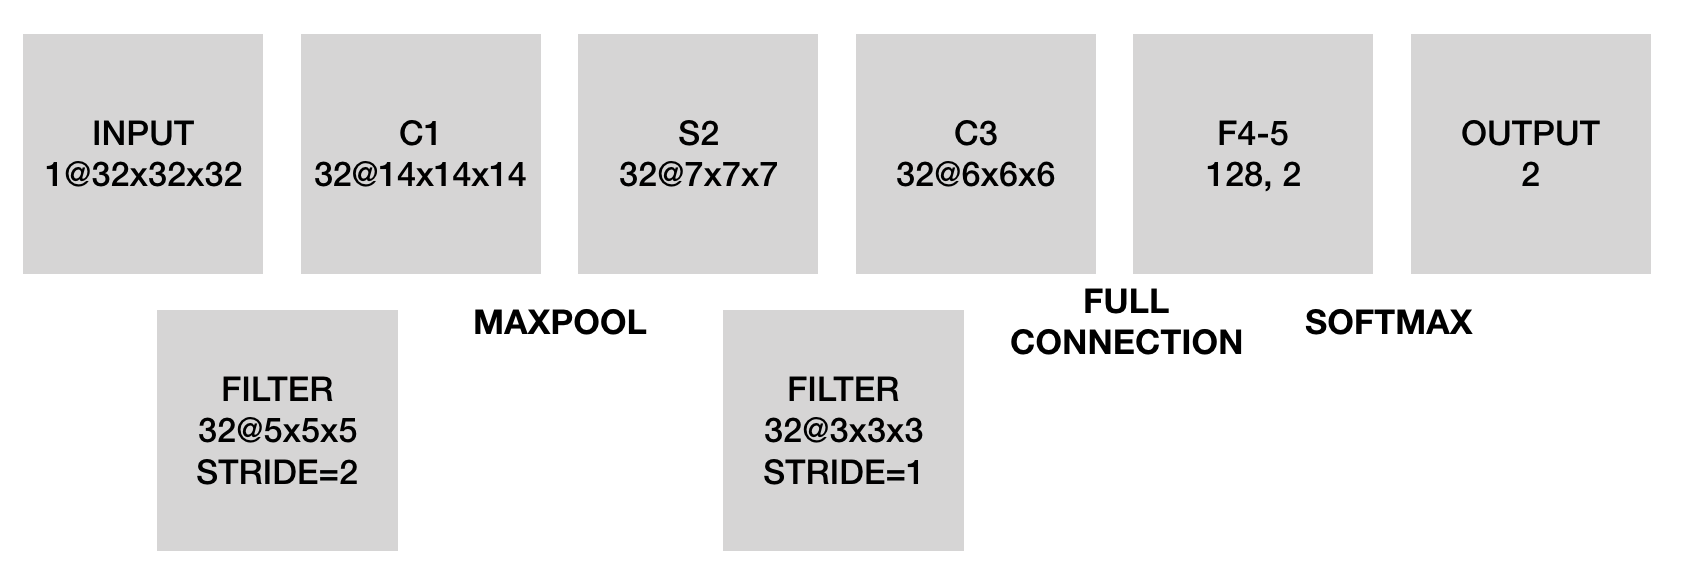
\includegraphics[width=8cm]{images/3DCNN.png}
    \caption{Structure of 3DCNN}
    \label{fig:my_label}
\end{figure}
The input is a 1 channel $32\times 32\times 32$ image from 3D occupancy grid representation. A $32\times 5 \times 5\times 5$ filter is applied with ${\rm stride}=2$ after the input layer, followed by a max pooling layer. The second filter is a $32\times 3\times 3\times3$ filter with ${\rm stride}=1$. After that, 2 full connection layer is applied and a Softmax function generates the output. Same as 2DCNN, this network also provide the probabilities of the input grasp being edge grasp and non-edge grasp.

\section{Experiments}
\subsection{Data Collection}
In order to train the CNNs, this paper firstly collect point cloud data from both simulator and real world, then use GPD \cite{RN6} to generate grasps. After that, the representation methods described above is applied to create images from grasps.

\subsubsection{Point Clouds.} A simulated shelf and a simulated depth sensor are created in OpenRAVE environment. The simulated camera takes the point cloud 20 times from 20 different positions, and combine them to 1 point cloud. 

For collecting real world point clouds, this paper used a UR5 robot arm with a depth sensor mounted on the wrist to collect data. For each point cloud, the robot goes to 2 view configurations and takes 2 point clouds. Then those 2 point clouds are combined into 1 point cloud. Points outside some work space (not reachable by the arm) is filtered out. 

\subsubsection{Grasps.} Point clouds are sent to GPD \cite{RN6} to generate potential grasps. After GPD returns a set of grasps, a filter is used to select grasps based on the geometry of the point cloud. For example, when generating data of table edge grasp, only the grasp candidates near the table edge will be selected. While when generating data of non-edge grasps on a table, grasps near the table edge will be filtered out. A grasp visualization method is used to visualize each group of selected grasp candidates to ensure that there are not too many noises. 

\subsubsection{Representation Images.} After a group of grasp candidates is selected, 2 representation algorithms described before will generate the input images. For each grasp, a 2D image and a 3D image is created. A binary label is used for all images, edge grasps will be labeled as 1 and non-edge grasps will be labeled as 0.

A total of 5842 grasp images is collected for each of the 2 neural nets. 3272 of them are labeled as edge grasps and others are labeled as non-edge grasps.

\subsection{Training}
\begin{figure}[!b]

\subfloat[Training Process of 2D CNN]{%
  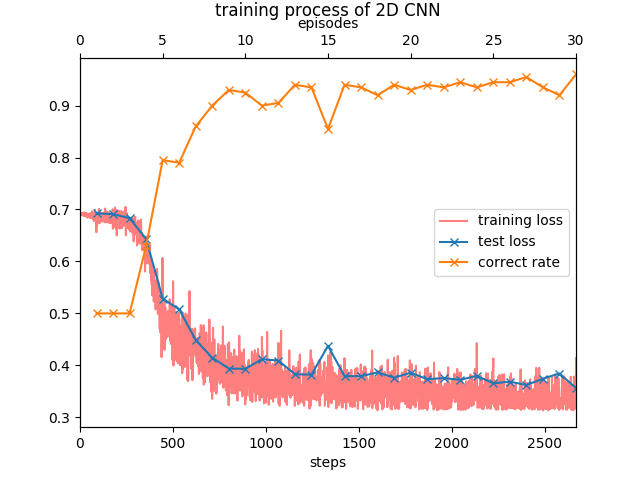
\includegraphics[width=\columnwidth]{images/2dtraining.png}%
}

\subfloat[Training Process of 3D CNN]{%
  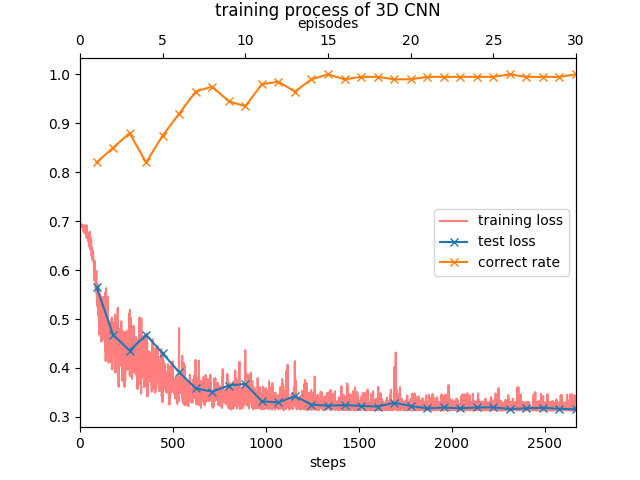
\includegraphics[width=\columnwidth]{images/3dtraining.png}%
}

\caption{Training process of 2 convolutional neural networks. Red: training loss for each training steps. Blue: validation loss for each training episodes. Orange: classification accuracy in validation set for each training episodes.}

\end{figure}
In both convolutional neural networks, this paper use same training parameters. Cross entropy loss is used as the loss function: 
\begin{equation}
    H(p, q)=-\sum_x p(x)\log q(x)
\end{equation}
where $p$ is the distribution of the label (one hot) and $q$ is the distribution of the output of the classifier.

Stochastic gradient descent is applied as the optimizer. The learning rate is 0.01, and batch size is 64. 

In the training process of 2D CNN, the classification accuracy converges at around 95\% after 16 training episodes (orange line in figure 4(a)). Both the test loss (blue line in figure 4(a)) and training loss (red line in figure 4(a)) decrease at the first 10 episodes, then remain relatively stable. 

In the training process of 3D CNN, the classification accuracy converges at around 98\% after 15 training episodes (orange line in figure 4(b)). The test loss (blue line in figure 4(b)) and training loss (red line in figure 4(b)) also decrease at the first 10 episodes. 

The performance of both 2D CNN and 3D CNN in the training process is good. By comparing the results, 3D CNN reaches a higher classification accuracy in the validation set, and has lower training loss and test loss throughout the training process. Also, the training loss of 3D CNN is more stable than that of the 2D CNN.

\subsection{Testing Trained Networks}
\begin{figure}[H]
    \centering
    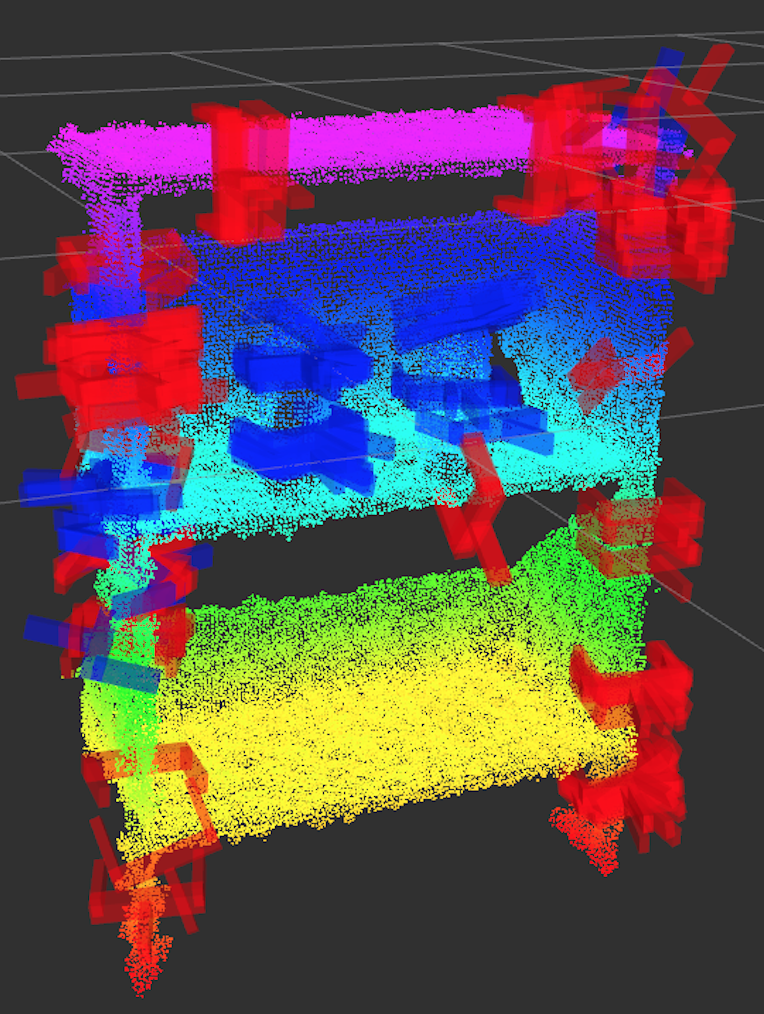
\includegraphics[width=8cm]{images/testexample.png}
    \caption{Visualization of Classification Results. Blue grasps are classified as non-edge grasps. Red grasps are classified as edge grasps.}
    \label{fig:my_label}
\end{figure}

\begin{figure}[H]
    \centering
    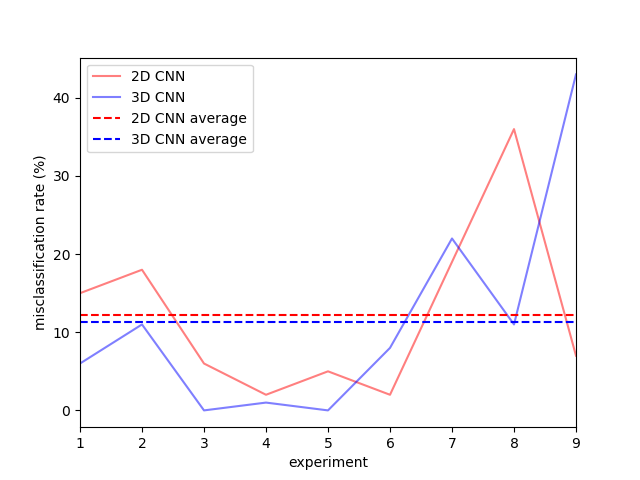
\includegraphics[width=\columnwidth]{images/exp1.png}
    \caption{Misclassification Rate. Red: 2D CNN. Blue: 3D CNN}
    \label{fig:my_label}
\end{figure}
The networks are tested on some new point clouds taken through the UR5 robot arm. After GPD generate potential grasps, the algorithm in this paper is used to classify edge grasps and non-edge grasps. Then the misclassified grasps are counted. As is shown in figure 6, the 2D CNN classifier has a misclassification rate of 12.2\% (average of 15\%, 18\%, 6\%, 2\%, 5\%, 2\%, 19\%, 36\%, 7\%), and the percentage for 3D CNN classifier is 11.3\% (average of 43\%, 11\%, 22\%, 8\%, 0\%, 1\%, 0\%, 11\%, 6\%).

\begin{figure}[H]
    \centering
    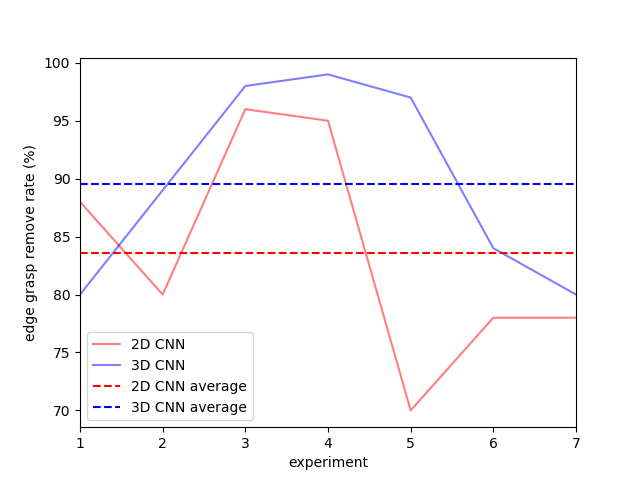
\includegraphics[width=\columnwidth]{images/exp2.png}
    \caption{Edge Grasp Removal. Red: 2D CNN. Blue: 3D CNN}
    \label{fig:my_label}
\end{figure}

Another experiment is made by testing how many percentages of edge grasps could be removed from all grasps candidates from GPD. As is shown in figure 7, 2D CNN classifier can remove 83.6\% edge grasps (average of 88\%, 80\%, 96\%, 95\%, 70\%, 78\%, 78\%). 3D CNN classifier can remove 89.6\% edge grasps (average of 80\%, 84\%, 97\%, 99\%, 98\%, 89\%, 80\%).



By comparing the performance of 3D CNN and 2D CNN, 3D CNN is more promising.



\section{Conclusion}
In this work, I finished a classifier that take point cloud and potential grasps as input, classify each grasp as edge grasp or non-edge grasp. The promising results show that both the 2D classifier and 3D classifier works well.

However, there are some drawbacks inside my project. Firstly, the data set is not big enough to produce a stable result, and this leads that the result of some experiments is not good enough. One experiment of 3D CNN has a misclassification rate of 43\%. Secondly, the environment inside this project is mainly inside the lab. There are only limited kinds of table and shelf, which means that the classifier may only perform well with similar tables and shelves.

\bibliographystyle{aaai}
\bibliography{lib}
\end{document}